\documentclass{standalone}
\usepackage{tikz}
\usetikzlibrary{patterns, positioning}
\usepackage[sfdefault]{ClearSans} %% option 'sfdefault' activates Clear Sans as the default text font
\usepackage[T1]{fontenc}

\begin{document}
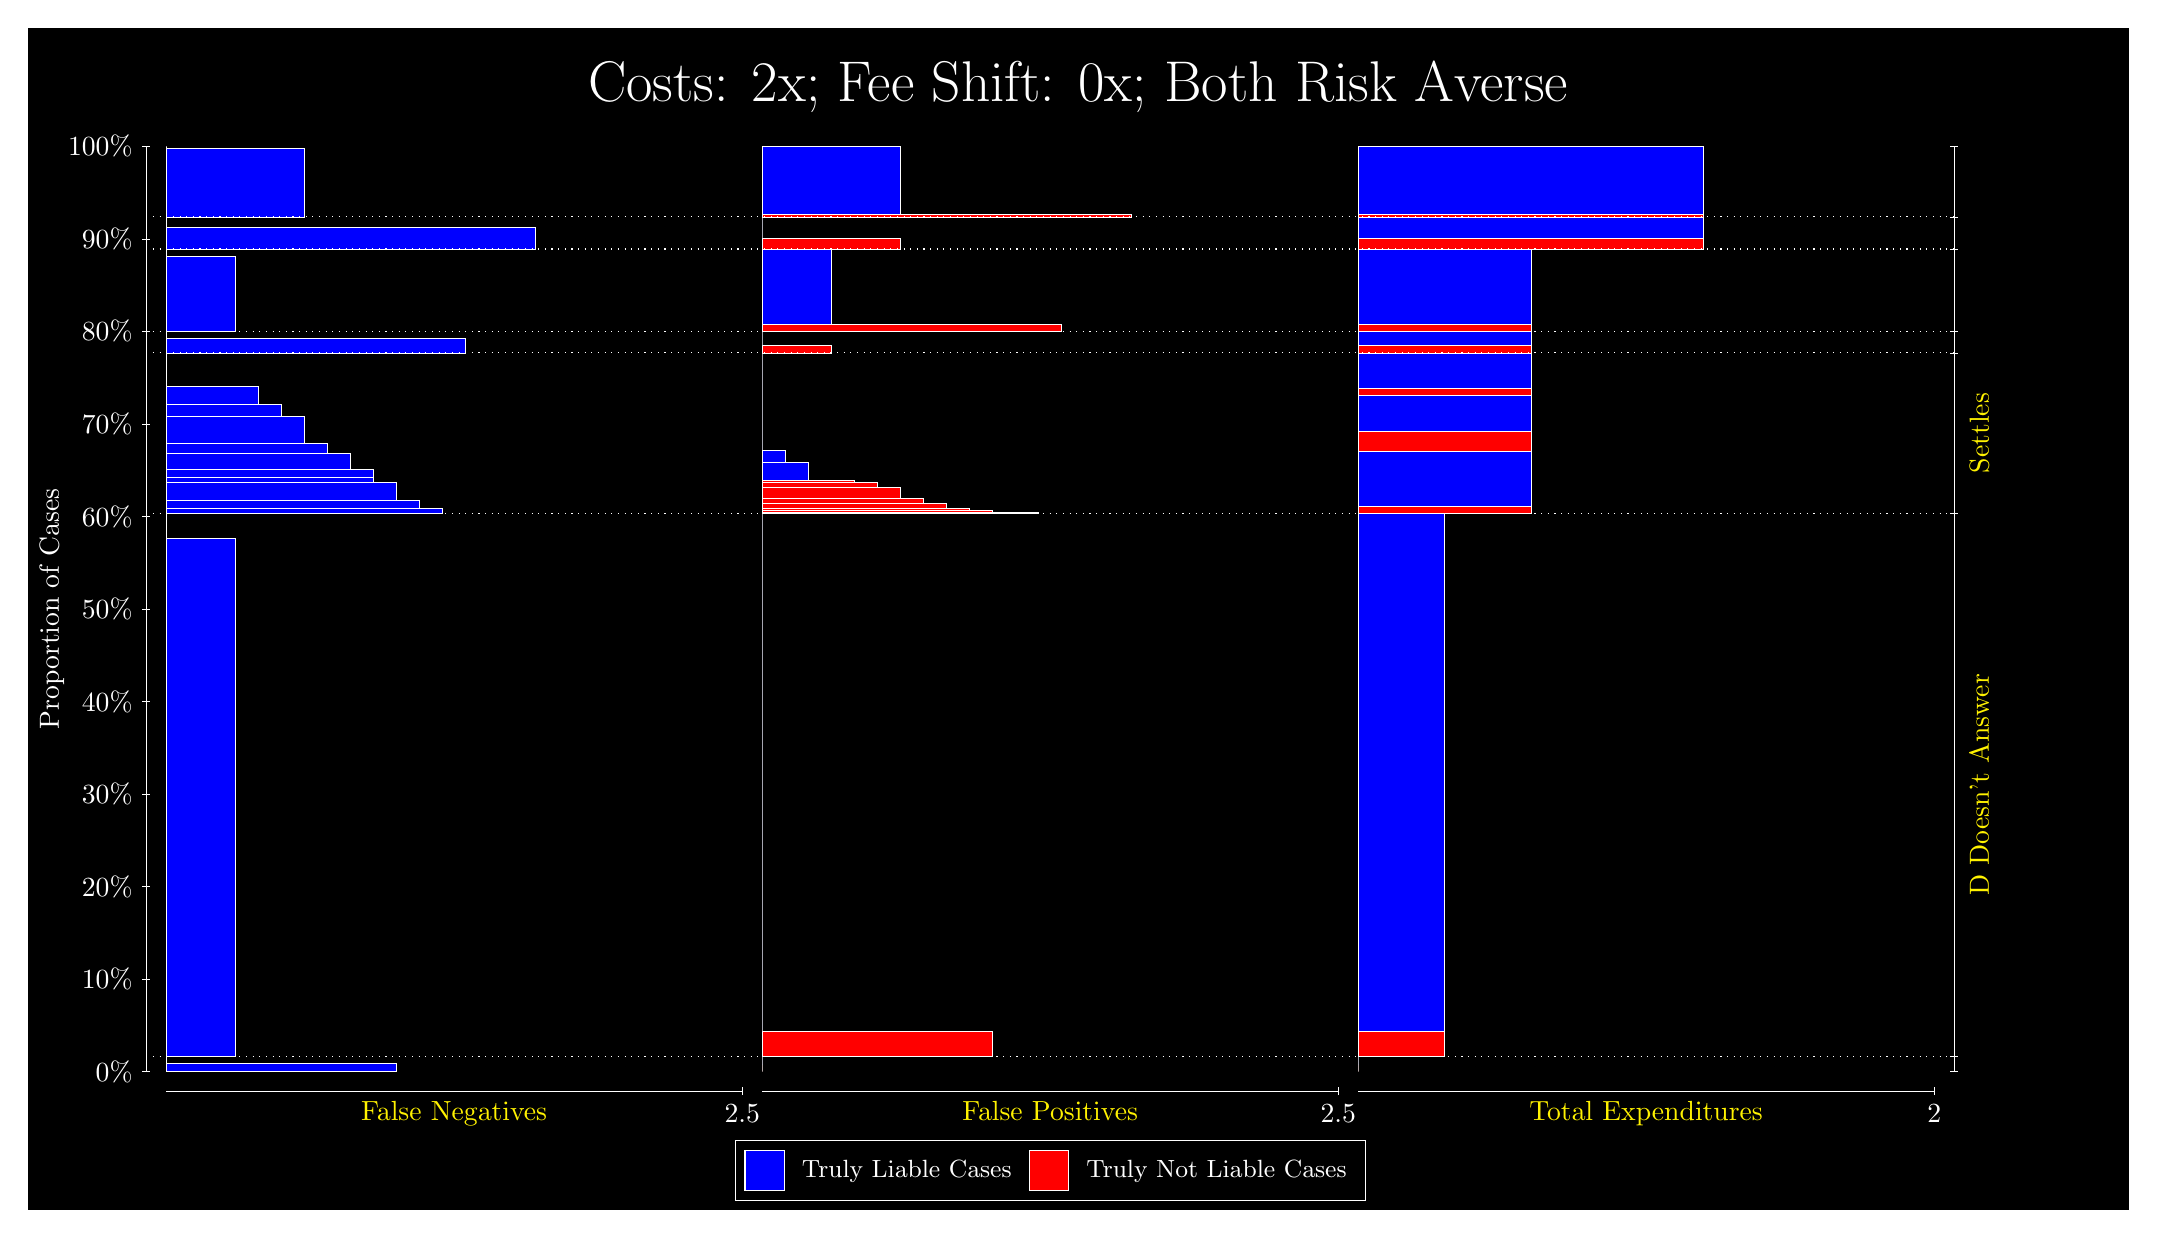
\begin{tikzpicture}
\draw[fill=black] (0,0) rectangle (26.667,15);
\draw[text=white] (0,13.5) rectangle (26.667,15) node[midway] {\huge Costs: 2x; Fee Shift: 0x; Both Risk Averse};
\draw[white, very thin] (1.5,1.75) -- (1.5,13.5);
\node[rotate=90, text=white, anchor=center] at (0.3, 7.625) {Proportion of Cases};
\draw[white, very thin] (1.45,1.75) -- (1.55,1.75);
\node[text=white, anchor=east] at (1.45, 1.75) {0\%};
\draw[white, very thin] (1.45,2.925) -- (1.55,2.925);
\node[text=white, anchor=east] at (1.45, 2.925) {10\%};
\draw[white, very thin] (1.45,4.1) -- (1.55,4.1);
\node[text=white, anchor=east] at (1.45, 4.1) {20\%};
\draw[white, very thin] (1.45,5.275) -- (1.55,5.275);
\node[text=white, anchor=east] at (1.45, 5.275) {30\%};
\draw[white, very thin] (1.45,6.45) -- (1.55,6.45);
\node[text=white, anchor=east] at (1.45, 6.45) {40\%};
\draw[white, very thin] (1.45,7.625) -- (1.55,7.625);
\node[text=white, anchor=east] at (1.45, 7.625) {50\%};
\draw[white, very thin] (1.45,8.8) -- (1.55,8.8);
\node[text=white, anchor=east] at (1.45, 8.8) {60\%};
\draw[white, very thin] (1.45,9.975) -- (1.55,9.975);
\node[text=white, anchor=east] at (1.45, 9.975) {70\%};
\draw[white, very thin] (1.45,11.15) -- (1.55,11.15);
\node[text=white, anchor=east] at (1.45, 11.15) {80\%};
\draw[white, very thin] (1.45,12.325) -- (1.55,12.325);
\node[text=white, anchor=east] at (1.45, 12.325) {90\%};
\draw[white, very thin] (1.45,13.5) -- (1.55,13.5);
\node[text=white, anchor=east] at (1.45, 13.5) {100\%};

\draw[white, very thin] (24.457,1.75) -- (24.457,13.5);
\draw[white, very thin] (24.407,1.75) -- (24.507,1.75);
\node[anchor=west] at (24.407, 1.75) {};
\draw[white, very thin] (24.407,1.9408) -- (24.507,1.9408);
\node[anchor=west] at (24.407, 1.9408) {};
\draw[white, very thin] (24.407,8.8389) -- (24.507,8.8389);
\node[anchor=west] at (24.407, 8.8389) {};
\draw[white, very thin] (24.407,10.878) -- (24.507,10.878);
\node[anchor=west] at (24.407, 10.878) {};
\draw[white, very thin] (24.407,11.15) -- (24.507,11.15);
\node[anchor=west] at (24.407, 11.15) {};
\draw[white, very thin] (24.407,12.196) -- (24.507,12.196);
\node[anchor=west] at (24.407, 12.196) {};
\draw[white, very thin] (24.407,12.605) -- (24.507,12.605);
\node[anchor=west] at (24.407, 12.605) {};
\draw[white, very thin] (24.407,13.5) -- (24.507,13.5);
\node[anchor=west] at (24.407, 13.5) {};

\draw[white, very thin, fill=blue] (1.75,1.75) rectangle (4.6775,1.8563);
\draw[white, very thin, fill=red] (1.75,1.8563) rectangle (1.75,1.9408);
\draw[white, very thin, fill=blue] (1.75,1.9408) rectangle (2.6283,8.5237);
\draw[white, very thin, fill=red] (1.75,8.5237) rectangle (1.75,8.8389);
\draw[white, very thin, fill=blue] (1.75,8.8389) rectangle (5.2631,8.9032);
\draw[white, very thin, fill=blue] (1.75,8.9032) rectangle (4.9703,9.0026);
\draw[white, very thin, fill=blue] (1.75,9.0026) rectangle (4.6775,9.2355);
\draw[white, very thin, fill=blue] (1.75,9.2355) rectangle (4.3848,9.2953);
\draw[white, very thin, fill=blue] (1.75,9.2953) rectangle (4.3848,9.4023);
\draw[white, very thin, fill=blue] (1.75,9.4023) rectangle (4.092,9.605);
\draw[white, very thin, fill=blue] (1.75,9.605) rectangle (3.7993,9.7307);
\draw[white, very thin, fill=blue] (1.75,9.7307) rectangle (3.5065,10.072);
\draw[white, very thin, fill=blue] (1.75,10.072) rectangle (3.2138,10.227);
\draw[white, very thin, fill=blue] (1.75,10.227) rectangle (2.921,10.452);
\draw[white, very thin, fill=red] (1.75,10.452) rectangle (1.75,10.878);
\draw[white, very thin, fill=blue] (1.75,10.878) rectangle (5.5558,11.061);
\draw[white, very thin, fill=red] (1.75,11.061) rectangle (1.75,11.15);
\draw[white, very thin, fill=blue] (1.75,11.15) rectangle (2.6283,12.104);
\draw[white, very thin, fill=red] (1.75,12.104) rectangle (1.75,12.196);
\draw[white, very thin, fill=blue] (1.75,12.196) rectangle (6.4341,12.466);
\draw[white, very thin, fill=red] (1.75,12.466) rectangle (1.75,12.605);
\draw[white, very thin, fill=blue] (1.75,12.605) rectangle (3.5065,13.47);
\draw[white, very thin, fill=red] (1.75,13.47) rectangle (1.75,13.5);
\draw[white, very thin, fill=red] (9.3189,1.75) rectangle (9.3189,1.8345);
\draw[white, very thin, fill=blue] (9.3189,1.8345) rectangle (9.3189,1.9408);
\draw[white, very thin, fill=red] (9.3189,1.9408) rectangle (12.246,2.256);
\draw[white, very thin, fill=blue] (9.3189,2.256) rectangle (9.3189,8.8389);
\draw[white, very thin, fill=red] (9.3189,8.8389) rectangle (12.832,8.8464);
\draw[white, very thin, fill=red] (9.3189,8.8464) rectangle (12.539,8.8536);
\draw[white, very thin, fill=red] (9.3189,8.8536) rectangle (12.246,8.8746);
\draw[white, very thin, fill=red] (9.3189,8.8746) rectangle (11.954,8.9007);
\draw[white, very thin, fill=red] (9.3189,8.9007) rectangle (11.661,8.9614);
\draw[white, very thin, fill=red] (9.3189,8.9614) rectangle (11.368,9.0293);
\draw[white, very thin, fill=red] (9.3189,9.0293) rectangle (11.075,9.17);
\draw[white, very thin, fill=red] (9.3189,9.17) rectangle (10.783,9.2295);
\draw[white, very thin, fill=red] (9.3189,9.2295) rectangle (10.49,9.2651);
\draw[white, very thin, fill=blue] (9.3189,9.2651) rectangle (9.9044,9.4898);
\draw[white, very thin, fill=blue] (9.3189,9.4898) rectangle (9.6116,9.645);
\draw[white, very thin, fill=blue] (9.3189,9.645) rectangle (9.3189,10.878);
\draw[white, very thin, fill=red] (9.3189,10.878) rectangle (10.197,10.967);
\draw[white, very thin, fill=blue] (9.3189,10.967) rectangle (9.3189,11.15);
\draw[white, very thin, fill=red] (9.3189,11.15) rectangle (13.125,11.242);
\draw[white, very thin, fill=blue] (9.3189,11.242) rectangle (10.197,12.196);
\draw[white, very thin, fill=red] (9.3189,12.196) rectangle (11.075,12.334);
\draw[white, very thin, fill=blue] (9.3189,12.334) rectangle (9.3189,12.605);
\draw[white, very thin, fill=red] (9.3189,12.605) rectangle (14.003,12.635);
\draw[white, very thin, fill=blue] (9.3189,12.635) rectangle (11.075,13.5);
\draw[white, very thin, fill=red] (16.888,1.75) rectangle (16.888,1.8345);
\draw[white, very thin, fill=blue] (16.888,1.8345) rectangle (16.888,1.9408);
\draw[white, very thin, fill=red] (16.888,1.9408) rectangle (17.986,2.256);
\draw[white, very thin, fill=blue] (16.888,2.256) rectangle (17.986,8.8389);
\draw[white, very thin, fill=red] (16.888,8.8389) rectangle (19.083,8.9278);
\draw[white, very thin, fill=blue] (16.888,8.9278) rectangle (19.083,9.627);
\draw[white, very thin, fill=red] (16.888,9.627) rectangle (19.083,9.8753);
\draw[white, very thin, fill=blue] (16.888,9.8753) rectangle (19.083,10.332);
\draw[white, very thin, fill=red] (16.888,10.332) rectangle (19.083,10.421);
\draw[white, very thin, fill=blue] (16.888,10.421) rectangle (19.083,10.878);
\draw[white, very thin, fill=red] (16.888,10.878) rectangle (19.083,10.967);
\draw[white, very thin, fill=blue] (16.888,10.967) rectangle (19.083,11.15);
\draw[white, very thin, fill=red] (16.888,11.15) rectangle (19.083,11.242);
\draw[white, very thin, fill=blue] (16.888,11.242) rectangle (19.083,12.196);
\draw[white, very thin, fill=red] (16.888,12.196) rectangle (21.279,12.334);
\draw[white, very thin, fill=blue] (16.888,12.334) rectangle (21.279,12.605);
\draw[white, very thin, fill=red] (16.888,12.605) rectangle (21.279,12.635);
\draw[white, very thin, fill=blue] (16.888,12.635) rectangle (21.279,13.5);
\draw[white, dotted] (1.5,1.9408) -- (24.457,1.9408);
\draw[white, dotted] (1.5,8.8389) -- (24.457,8.8389);
\draw[white, dotted] (1.5,10.878) -- (24.457,10.878);
\draw[white, dotted] (1.5,11.15) -- (24.457,11.15);
\draw[white, dotted] (1.5,12.196) -- (24.457,12.196);
\draw[white, dotted] (1.5,12.605) -- (24.457,12.605);
\draw[white, very thin] (1.75,1.5) -- (9.0689,1.5);
\node[text=yellow, anchor=north] at (5.4094, 1.5) {False Negatives};
\draw[white, very thin] (9.0689,1.45) -- (9.0689,1.55);
\node[text=white, anchor=north] at (9.0689, 1.45) {2.5};

\draw[white, very thin] (9.3189,1.5) -- (16.638,1.5);
\node[text=yellow, anchor=north] at (12.978, 1.5) {False Positives};
\draw[white, very thin] (16.638,1.45) -- (16.638,1.55);
\node[text=white, anchor=north] at (16.638, 1.45) {2.5};

\draw[white, very thin] (16.888,1.5) -- (24.207,1.5);
\node[text=yellow, anchor=north] at (20.547, 1.5) {Total Expenditures};
\draw[white, very thin] (24.207,1.45) -- (24.207,1.55);
\node[text=white, anchor=north] at (24.207, 1.45) {2};


\node[text=yellow, centered, rotate=90] at (24.777, 5.3899) {D Doesn't Answer};
\node[text=yellow, centered, rotate=90] at (24.777, 9.8585) {Settles};





\draw (12.978300999999998,1.5) node[draw=none] (baseCoordinate) {};
\begin{scope}[align=center]
        \matrix[scale=0.5, draw=white, below=0.5cm of baseCoordinate, nodes={draw}, column sep=0.1cm]{
            \node[rectangle, draw, minimum width=0.5cm, minimum height=0.5cm, fill=blue] {}; &
            \node[draw=none, font=\small, text=white] (B) {Truly Liable Cases}; &
            \node[rectangle, draw, minimum width=0.5cm, minimum height=0.5cm, fill=red] {}; &
            \node[draw=none, font=\small, text=white] (B) {Truly Not Liable Cases}; \\
            };
\end{scope}

\end{tikzpicture}
\end{document}